\chapter{Schnorr: Identificazione e Firma Digitale}

In questo capitolo verranno presentati i protocolli di Zero-Knowledge Proof (ZKP), introdotti per la prima volta alla fine degli anni '80 da Shafi Goldwasser, Silvio Micali e Charles Rackoff nel documento \textit{The Knowledge Complexity of Interactive Proof-Systems}\cite{doi:10.1137/0218012}. Particolare attenzione sarà dedicata al \textbf{protocollo di identificazione di Schnorr} e al corrispondente \textbf{schema di firma digitale}.

\section{Protocolli "Zero Knowledge Proof"}\label{sec:zkp}

\begin{de}[Zero-Knowledge-Proof Protocol] 
	Un protocollo conosciuto nella crittografia come \textit{Zero-Knowledge-Proof Protocol} (indicato con ZK oppure ZKP) rappresenta uno schema di dimostrazione nel quale un soggetto, detto \textbf{Prover}, deve convincere un secondo soggetto, detto \textbf{Verifier}, che una \textbf{dichiarazione} chiamata è vera, senza dover offrire informazioni aggiuntive riguardo il\textbf{testimone segreto (Witness)} che la rende vera.
\end{de}

L'intuizione alla base della dimostrazione a conoscenza zero è che è banale convincere del possesso di informazioni sensibili semplicemente rivelandole, mentre risulta più complesso  dimostrare il possesso di tali informazioni senza dover rivelarle.

Le dimostrazioni a conoscenza zero possono essere interattive, infatti tra Prover e Verifier si crea una comunicazione nella quale si effettua uno scambio di messaggi secondo un protocollo ben determinato. Esistono anche dimostrazioni a conoscenza zero non interattive, nelle quali il Prover convince il Verifier inviando un solo messaggio.

Al fine di chiarire meglio il funzionamento dei protocolli ZKP, si consideri il seguente esempio astratto.

Si tratta di una storia che racchiude al meglio i principi fondamentali delle dimostrazioni a conoscenza zero. È stato presentato per la prima volta da Jean-Jacques Quisquater in \cite{10.1007/0-387-34805-0_60}.

L’esempio, noto come storia della caverna di Alì Babà, descrive una situazione in cui un Prover (Peggy) deve convincere un Verifier (Victor) di conoscere un segreto (la parola magica che apre una porta nella caverna), senza però rivelarlo direttamente.

In questa storia, Peggy, è in possesso della parola segreta in grado di aprire una porta magica in una caverna. La caverna è a forma di anello con l'ingresso da una parte e, dal lato opposto, la porta magica che impedisce il passaggio da un percorso all'altro come mostrato in \autoref{fig:ali_baba_cave}. Victor vuole sapere se Peggy conosce o meno la parola segreta ma Peggy essendo una persona riservata, non vuole rivelare a Victor la parola magica. I percorsi sono etichettati con A (sinistro) e B (destro). Victor aspetta all'entrata mentre Peggy sceglie quale percorso usare senza che Victor lo sappia. Dopodiché, Victor entra nella caverna e grida quale percorso - scelto a caso - deve usare Peggy per fare ritorno all'entrata. A patto che conosca davvero la parola magica, sarebbe facile: aprirebbe la porta, se necessario, per tornare indietro seguendo il percorso desiderato.

% TODO: MODIFICARE LA CITAZIONE

Tuttuvia, supponendo che Peggy non conosca la parola magica, avrebbe potuto fare ritorno usando il percorso indicato solo se Victor avesse scelto il percorso seguito inizialmente da Peggy. Siccome Victor sceglie casualmente il percorso, lei ha il $50\%$ di probabilità di indovinare correttamente il percorso da seguire per fare ritorno. Se questo processo viene ripetuto, diciamo, 20 volte, allora la probabilità di successo, ovvero di anticipare correttamente la richiesta di Victor, si ridurrebbe a $\frac{1}{2^{20}}$.

In conclusione, se Peggy ripetutamente appare all'entrata seguendo il percorso scelto da Victor, allora si può concludere che Peggy conosce la parola magica.

\begin{figure}[h!]
	\centering
	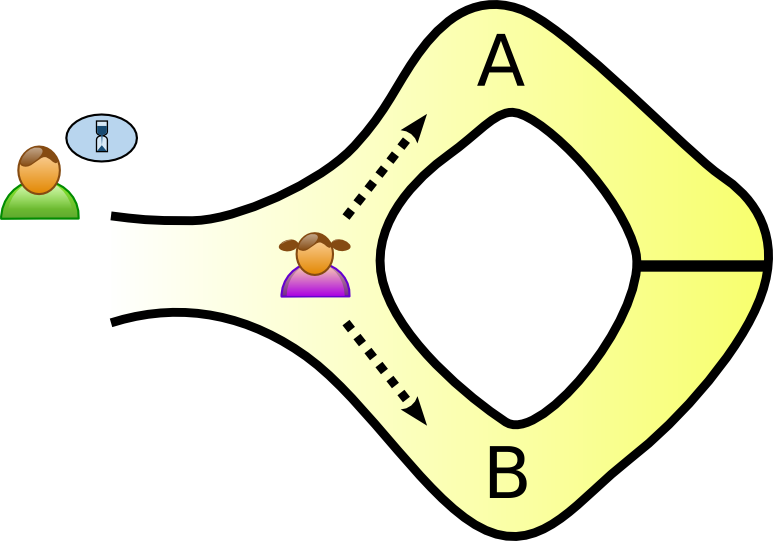
\includegraphics[width=0.6\textwidth]{images/ali_baba_cave.png}
	\caption{Rappresentazione della caverna di Alì Babà.}
	\label{fig:ali_baba_cave}
\end{figure}

Ora che è stato chiarito meglio il funzionamento dei protocolli ZKP, si piò procedere con elencare le tre proprietà che una dimostrazione ZKP deve soddisfare.

\subsection{Proprietà}\label{sec:zkp-prop}

\begin{enumerate}
	\item \textbf{Completezza}: Se l'affermazione è vera, allora un verificatore onesto sarà convinto di questo fatto da un dimostratore onesto.
	\item \textbf{Correttezza}: Se l'affermazione è falsa, allora nessun dimostratore può imbrogliare un verificatore onesto che il fatto è vero, o meglio la probabilità di riuscire a convincerlo può essere ridotta a piacimento.
	\item \textbf{Zero Knowledge Proof}: Se l'affermazione è vera, allora nessun verificatore è in grado di acquisire informazioni aggiuntive oltre al fatto che l'affermazione è vera. 
\end{enumerate}

La ricerca nell'ambito dei protocolli ZKP ha portato allo sviluppo di sistemi di autenticazione a conoscenza zero, in cui un'entità prova a dimostrare la propria identità ad un'altra entità tramite un'informazione segreta (es. password) senza rivelare tale informazione. Questo tipo di autenticazione è chiamato "Zero Knowledge - Proof of Knowledge" (prova di conoscenza a conoscenza zero).

Per implementare tali protocolli in modo efficiente e sicuro sono stati sviluppati diversi schemi formali. Tra i più studiati e applicati troviamo i cosiddetti \textit{$\Sigma$-Protocols}\footnote{Il protocollo d'identificazione di Schnorr è un caso speciale di Sigma Protocol ed è oggetto di studio di questa tesi.}, che costituiscono una classe di protocolli interattivi a tre mosse (commitment, challenge, response) particolarmente adatti alla costruzione di prove di conoscenza a conoscenza zero. 

\newpage

\section{Protocolli Sigma}

In questa sezione si andrà a discutere dei protocolli $\Sigma$\footnote{Letto \textit{Sigma}, dove la prima parte richiama lo "zig-zag" delle tre mosse tipiche di un protocollo interattivo, mentre il suffisso è un'abbreviazione di "Merlin-Artur".} introdotti per la prima volta da R. Cramer nella sua tesi di dottorato \cite{pub:21438}. In particolare verrà data una definizione di cos'è un protocollo Sigma, di come funziona e quali sono le proprietà fondamentali. L'argomento è trattato con maggiori dettagli nel libro D. Boneh and V. Shoup, \textit{A Graduate Course in Applied Cryptography}, Cap. 19.4 \cite{boneh2020applied}.

\begin{de}[Relazione Effettiva] Una \textbf{relazione effettiva} è una relazione binaria $\mathcal{R} \subseteq \mathcal{X} \times \mathcal{Y}$, dove $\mathcal{X},\ \mathcal{Y} \text{ e } \mathcal{R}$ sono degli insiemi finiti riconoscibili in modo efficiente. Gli elementi di $\mathcal{Y}$ sono detti \textbf{affermazioni (statements)}. Se $(x, y) \in \mathcal{R}$, allora $x$ è detto \textbf{testimone per (witness for)} $y$.
\end{de}

\begin{de}[Protocollo Sigma]\label{def:sigma} Sia $\mathcal{R} \subseteq \mathcal{X} \times \mathcal{Y}$ una relazione effettiva. Un \textbf{Protocollo Sigma} su $\mathcal{R}$ è una coppia $(P, V)$.
	\begin{itemize}[itemsep=0.3em, topsep=0.2em]
		\item $P$ è un protocollo interattivo chiamato \textbf{prover}, e prende in input una coppia \textit{testimone-affermazione} $(x, y) \in \mathcal{R}$.
		\item $V$ è un protocollo interattivo chiamato \textbf{verifier}, prende in input un'\textit{affermazione} $y \in \mathcal{Y}$ ($V$ non è a conoscenze del testimone $x$), e restituisce in output \textit{accetta} o \textit{rigetta}.
		\item $P$ e $V$ sono strutturati in modo che un'interazione tra loro avvenga nel seguente modo (vedere \autoref{fig:sigma-protocol}):
		      \begin{itemize}[itemsep=0.1em, topsep=0.2em]
		      	\item Per iniziare, $P$ computa un messaggio $t$, chiamato \textbf{commitment}, e lo invia a $V$.
		      	\item Una volta ricevuto il messaggio $t$ da $P$, $V$ sceglie casualmente un valore $c$, chiamato \textbf{challenge}, da uno spazio finito $\mathcal{C}$, detto \textbf{challenge space}, e lo invia a $P$.
		      	\item Una volta ricevuta la challenge $c$ da $V$, $P$ computa  $z$, detto \textbf{response}, e lo invia a $V$.
		      	\item Ricevuto $z$, $V$ decide se \textit{accettare} o \textit{rigettare} dopo aver calcolato una funzione dipendente dall'affermazione $y$ e dalla conversazione (\textbf{conversation}) $(t, c, z)$.
		      	              
		      	      In particolare, $V$ non effettua ulteriori scelte casuali se non per scegliere $c$, il resto delle computazioni sono strettamente \textit{deterministiche}. 
		      \end{itemize}
	\end{itemize}
\end{de}

\newpage

\begin{figure}[h!]
	\centering
	\begin{tikzpicture}[>=latex, font=\small]
		
		\node (P) at (-3,0) {$\underline{P(x, y)}$};
		\node (V) at (4,0) {$\underline{V(y)}$};
		
		\node[left] at (-3,-1) {\textit{commitment} $t$};
		\draw[->] (-3,-1.3) -- (4,-1.3) node[midway,above] {$t$};
		
		\node[right] at (4,-2) {\textit{challenge}: $c \;\overset{R}{\leftarrow}\; \mathcal{C}$};
		
		\draw[<-] (-3,-2.3) -- (4,-2.3) node[midway,below] {$c$};
		
		\node[left] at (-3,-3) {\textit{response} $z$};
		\draw[->] (-3,-3.3) -- (4,-3.3) node[midway,above] {$z$};
		
		\node[right] at (4,-3.6) {\textit{accetta/rigetta}};
		
	\end{tikzpicture}
	\caption{Schema di un protocollo $\Sigma$ interattivo}
	\label{fig:sigma-protocol}
\end{figure}
\hrulefill

Come specificato nella \autoref{def:sigma}, è richiesto che il verifier calcoli una funzione 
$$f :  (y, t, c, z) \to \{\textit{accetta}, \textit{rigetta}\},$$
dipendente da $y$ e dalla conversazione $(t, c, z)$.
Se l'esisto della funzione è \textit{accetta}, allora la conversazione $(t, c, z)$ è detta \textbf{accettata per} $y$.

È chiaro che un'interazione tra un verifier e un prover \textit{onesto} porti sempre ad una conversazione accetata. Conversazioni rigettate si verificano, ad esempio, quando il verifier interagisce con un prover \textit{disonesto} che non rispetta il protocollo concordato.

Inoltre, in molte applicazioni dei protocolli Sigma è richiesto che lo spazio delle challenge $\mathcal{C}$ sia super-poly\footnote{Nella teoria della complessità, quando si parla di \textbf{super-poly space} si intende uno spazio di memoria che cresce più velocemente di qualunque polinomio nella dimensione dell'input.}.

\subsection{Proprietà}\label{sec:sigma-prop}

I protocolli $\Sigma$ si inseriscono nella categoria dei Zero-Knowledge-Proof e, di conseguenza, rispettano tutte e tre le proprietà fondamentali già elencate nella \autoref{sec:zkp-prop}. Tuttavia, queste vengono formulate in maniera più specifica, dando origine alle nozioni di \textbf{perfect completeness}, \textbf{special soundness} e \textbf{special honest-verifier zero-knowledge (HVZK)}.

\begin{itemize}
	\item \textbf{Perfect Completeness}: $\forall (x, y) \in \mathcal{R}$, quando $P(x, y)$ e $V(y)$ interagiscono tra loro, $V(y)$ deve \textit{accettare} sempre. Formalmente, abbiamo che:
	      $$\forall (x, y) \in \mathcal{R},\ \Pr \left[\langle P(x, y), V(y) \rangle =\ accetta \right] = 1$$
	      dove $\langle P(x, y), V(y) \rangle$ rappresenta l'interazione tra $V$ e $P$.
	\item \textbf{Special Soundness}: Sia $(P, V)$ un protocollo Sigma per la relazione $\mathcal{R} \subseteq \mathcal{X} \times \mathcal{Y}$. Si dice che $(P, V)$ offre una solidità speciale (\textbf{special soundness}) se esiste un algoritmo deterministico efficiente \textit{Ext}, chiamato estrattore di testimoni (\textbf{witness extractor}), avente la seguente proprietà: ogni volta che ad \textit{Ext} viene fornito in input un'affermazione $y \in \mathcal{Y}$ e due conversazioni di accettazione $(t, c, z)$ e $(t, c', z')$, con $c \neq c'$, l'algoritmo restituisce sempre in output $x \in \mathcal{X}$ tale che $(x, y) \in \mathcal{R}$, dove $x$ è il testimone di $y$.
	\item \textbf{Special HVZK}: Sia $(P, V)$ un protocollo Sigma per la relazione $\mathcal{R} \subseteq \mathcal{X} \times \mathcal{Y}$ con spazio delle sfide $\mathcal{C}$. Si dice che $(P, V)$ è un verificatore onesto a conoscenza zero (\textbf{special HVZK}), se esiste un algoritmo probabilistico efficiente \textit{Sim}, chiamato \textbf{simulatore}, che prende in input $(y, c) \in \mathcal{Y} \times \mathcal{C}$ avente le seguenti proprietà:
	      \begin{enumerate}
	      	\item Per ogni input $(y, c) \in \mathcal{Y} \times \mathcal{C}$, l'algoritmo \textit{Sim} produce in output una coppia $(t, z)$ tale che $(t, c, z)$ è una conversazione accettata per $y$.
	      	\item Per ogni $(x, y) \in \mathcal{R}$, se si calcola
	      	      $$c \overset{R}{\leftarrow} \mathcal{C},\ (t, z) \overset{R}{\leftarrow} Sim(y, c),$$
	      	      allora $(t, c, z)$ ha la stessa distribuzione di quella di una trascrizione di una conversazione tra $P(x, y)$ e $V(y)$.
	      	      
	      	      In altre parole, questa proprietà dice che, dato un protocollo Sigma $(P, V)$ per $\mathcal{R} \subseteq \mathcal{X} \times \mathcal{Y}$ e sia la coppia $(x, y) \in \mathcal{R}$, una conversazione tra $P(x, y)$ e $V(y)$ non rivela alcuna informazione aggiuntiva riguardo al testimone $x$.
	      \end{enumerate}
\end{itemize}

A primo impatto, sembrerebbe che la \textbf{special soundness} sia una proprietà indesiderabile: Perché vorremmo una proprietà che ci permette di estrarre il testimone $x$, date due conversazioni accettate?
Innanzitutto, è importante osservare che la definizione vale soltanto se le due conversazioni condividono lo stesso \textit{commitment} $t$ mentre le \textit{challenge} $c$ sono diverse. Infatti, possiamo dire che \textit{se qualcuno riesce a rispondere correttamente a due sfide diverse partendo dallo stesso $t$, allora deve "sapere qualcosa di vero" sul segreto}. Se $t$ fosse diverso, non avrebbe senso dire che "due risposte diverse rivelano il segreto": sarebbero due protocolli indipendenti. Inoltre, poiché $t$ viene scelto in modo casuale dal Prover, è improbabile che un \textit{honest Prover} invii due volte lo stesso $t$.
Quindi, il caso in cui il Verifier ottiene due conversazioni con lo stesso $t$ ma sfide diverse accade solo se il Prover è sotto il controllo dell'estrattore (come avviene nella definizione teorica di soundness).

In particolare, la \textbf{special soundness}, ci garantisce:
\begin{itemize}
    \item \textbf{Soundness}: Significa che un Prover che non conosce $x$ non può rispondere correttamente a più di una sfida, perché altrimenti sarebbe possibile estrarre $x$ dalle sue risposte.
    Di conseguenza, un truffatore che vuole ingannare il Verifier ha una probabilità di successo al massimo pari a: \[\frac{1}{|\mathcal{C}|}\].
    \item \textbf{Proof of Knowledge}: Consente di costruire un estrattore \textit{Ext}: un algoritmo che, interagendo con un Prover qualunque, può "riavvolgerlo" allo stato precedente alla ricezione della challenge $c$ (mantenendo lo stesso commitment $t$) e ottenere due conversazioni valide per estrarre il segreto $x$. Questo serve a formalizzare che il protocollo non dimostra solo che "l'affermazione è vera", ma che il Prover conosce effettivamente il testimone $x$. Se il Prover fosse uno non onesto, allora non sarebbe possibile generare due conversazioni valide "riavvolgendolo", in quanto per ipotesi, non conosce il testimone $x$.
\end{itemize}

\newpage

\section{Firme Digitali}\label{sec:sig-dig}

Una \textbf{firma digitale} è un meccanismo crittografico che permette di garantire \textbf{l'autenticità}, \textbf{l'integrità} e \textbf{la non ripudiabilità} di un documento o di un messaggio elettronico. Nello specifico, si vuole assicurare che un'informazione:
\begin{itemize}
    \item Provenga davvero dal mittente dichiarato (autenticità).
    \item Non sia stata alterata durante la trasmissione o l'archiviazione (integrità).
    \item Non possa essere negata dal mittente (non ripudiabilità).
\end{itemize}

Dal punto di vista tecnico, la firma digitale si basa sulla crittografia asimmetrica: ogni utente possiede una coppia di chiavi, una privata e una pubblica. La chiave pubblica viene utilizzata per generare la firma sul documento mentre la chiave privata viene usata dai destinatari per verificarne la validità. In pratica, il documento/messaggio non viene firmato direttamente, ma se ne calcola un hash. Questo hash viene poi cifrato con la chiave privata del mittente: il risultato è la firma digitale. Chi riceve il documento potrà ricalcolare l'hash e confrontarlo con quello decifrato usando la chiave pubblica del mittente: se coincidono, la firma è valida.

Le firme digitali sono oggi fondamentali in moltissimi contesti: posta elettronica certificata, documenti legali, contratti online, servizi bancari, e in generale in ogni scenario in cui sia necessario garantire sicurezza e fiducia nello scambio di informazioni.

Di seguito, una definizione formale di firma digitale ripresa da (D. Boneh and V. Shoup, \textit{A Graduate Course in Applied Cryptography}, Cap. 13.1 Pag 528 \cite{boneh2020applied}).
\begin{de}[Firma digitale]
    Un \textbf{sistema di firme digitali} $\mathcal{S} = (G,\ S,\ V)$ è una tripla di algoritmi efficienti, $G,\ S,\ V$, dove $G$ è chiamato \textbf{algoritmo di generazione delle chiavi}, $S$ è chiamato $\textbf{algoritmo di firma}$ e, infine, $V$ è detto \textbf{algoritmo di verifica}. Dunque, $S$ è usato per \textit{generare} le firme e $V$ è usato per \textit{verificare} le firme.
    Nello specifico,
    \begin{itemize}
        \item $G$ è un algoritmo \textit{probabilistico} che non richiede nessun input. Fornisce invece in output una coppia $(pk, sk)$, dove $sk$ è la \textbf{chiave segreta di firma} e $pk$ è la \textbf{chiave pubblica di verifica}.
        \item $S$ è anch'esso un algoritmo \textit{probabilistico} che ha il ruolo di computare 
        \[\sigma \overset{R}{\leftarrow} S(sk,\ m),\]
        dove $sk$ è la chiave segreta generata da $G$ ed $m$ è il messaggio. L'algoritmo restituisce in output la \textbf{firma} $\sigma$.
        \item $V$ è un algoritmo \textit{deterministico}, tale che 
        \[\texttt{accept or reject} \leftarrow V(pk,\ m,\ \sigma).\]
        \item È inoltre richiesto che la firma generata da $S$ sia sempre accettata da $V$. Ovvero, per ogni coppia $(pk. sk)$ generata da $G$ e per ogni messaggio $m$, si ha:
        \[\text{Pr}[V(pk,\ m,\ S(sk,\ m)) = \texttt{accept}] = 1.\]
    \end{itemize}
    Infine, diremo che i messaggi $m$ risiedono in uno \textbf{spazio di messaggi} finito $\mathcal{M}$ e le firme risiedono in uno \textbf{spazio di firme} finito $\Sigma$. Diremo inoltre che $\mathcal{S} = (G,\ S,\ V)$ è definito su $(\mathcal{M},\ \Sigma)$.
\end{de}

\subsection{Euristica di Fiat-Shamir per le Firme}\label{sec:fiat-shamir}

È possibile convertire protocolli Sigma in schemi di firma digitale usando una tecnica sviluppata da Fiat e Shamir conosciuta come \textbf{l'euristica di Fiat-Shamir} oppure come la \textbf{trasformazione di Fiat-Shamir} \cite{10.1007/3-540-47721-7_12}. Gli elementi costitutivi sono i seguenti:

\begin{itemize}
    \item Un protocollo Sigma $(P,\ V)$ definito per una relazione $\mathcal{R} \subseteq \mathcal{X} \times \mathcal{Y}$; assumiamo inoltre che le conversazioni siano della forma $(t,\ c,\ z)$, dove $t \in \mathcal{T},\ c \in \mathcal{C},\ z \in \mathcal{Z}$;
    \item Un algoritmo di generazione delle chiavi $G$ per $\mathcal{R}$;
    \item Una funzione hash $H: \mathcal{M} \times \mathcal{T} \rightarrow \mathcal{C}$, modellata come un'oracolo casuale; l'insieme $\mathcal{M}$ è lo spazio dei messaggi per lo schema di firme digitali.
\end{itemize}

Lo schema di firme di Fiat-Shamir derivato da $G$ e dal protocollo Sigma $(P, V)$ funziona nel seguente modo:

\begin{itemize}
    \item L'algoritmo di generazione delle chiavi è $G$, dunque, una chiave pubblica è della forma $pk = y$, dove $y \in \mathcal{Y}$ e una chiave segreta è della forma $sk = x$, dove $(x, y) \in \mathcal{R}$.
    \item Affinché possa firmare un messaggio $m \in \mathcal{M}$ usando una chiave segreta $sk = (x, y)$, l'algoritmo di firma deve funzionare nel seguente modo:
    \begin{itemize}
        \item Inizializza il prover $P(x, y)$, ottenendo il \textit{commitment} $t \in \mathcal{T}$;
        \item Calcola la \textit{challenge} $c \leftarrow H(m, t)$;
        \item Infine, immette $c$ nel prover, ottenendo una \textit{response} $z$ e restituendo in output la firma $\sigma := (t, z) \in \mathcal{T} \times \mathcal{Z}$. 
    \end{itemize}
    \item Per verificare la firma $\sigma = (t, z) \in \mathcal{T} \times \mathcal{Z}$ su un messaggio $m \in \mathcal{M}$ usando la chiave pubblica $pk = y$, l'algoritmo di verifica calcola $c \leftarrow H(m, t)$ e verifica che $(t, c, z)$ è una conversazione accettata per $y$.
\end{itemize}

\section{Protocollo d'Identificazione di Schnorr}\label{sec:schnorr}

Il paragrafo che segue è dedicato all'argomento principale di questa tesi: il \textbf{protocollo d'identificazione di Schnorr}, ideato da Claus Peter Schnorr alla fine degli anni '80 nel documento \textit{Efficient signature generation by smart cards}\cite{Schnorr2005}. È uno dei più celebri esempi di Sigma protocol basato sul problema del logaritmo discreto. La sua importanza risiede nel fatto che fornisce una base per numerosi schemi di autenticazione moderni e di firme digitali (\textbf{firma digitale di Schnorr}).

La struttura del protocollo segue il paradigma \textbf{commitment-challenge-response}, tipico dei Sigma protocol, rispettando tutte le proprietà fondamentali: \textbf{perfect completeness, special soundness, special HVZK}.

\begin{de}
	Sia $\mathbb{G}$ un gruppo ciclico di ordine primo $q$ con generatore $g \in \mathbb{G}$ e sia $\mathcal{C} \subseteq \mathbb{Z}_q$. Il protocollo d'identificazione di Schnorr è identificato dalla tripla $\mathcal{I}_{sch} = (G, P, V)$, dove:
	\begin{itemize}
		\item $G$ rappresenta l'algoritmo di generazione delle chiavi e funziona nel seguente modo:
		      $$\alpha \overset{R}{\leftarrow} \mathbb{Z}_q,\ u \leftarrow g^{\alpha}$$
		      La chiave di verifica è $vk := u$, mentre la chiave segreta $sk := \alpha$.
		\item $P$ è il prover inizializzato con $sk = \alpha$ mentre $V$ è il verifier inizializzato con $vk = u$. Il protocollo di comunicazione tra $P$ e $V$ è il seguente, come mostrato in \autoref{fig:schnorr-protocol}:
		      \begin{enumerate}
		      	\item $P$ calcola $\alpha_t \overset{R}{\leftarrow} \mathbb{Z}_q$, $u_t \leftarrow g^{\alpha_t}$, e invia $u_t$ a $V$;
		      	\item $V$ calcola $c \overset{R}{\leftarrow} \mathcal{C}$, e lo invia a $P$;
		      	\item $P$ calcola $\alpha_z \leftarrow \alpha_t + \alpha c \in \mathbb{Z}_q$, inviandolo poi a $V$;
		      	\item $V$ effettua il seguente controllo: $$g^{\alpha_z} = u_t \cdot u^c$$ Se l'uguaglianza è verificata allora $V$ \textit{accetta}, altrimenti \textit{rigetta}. 
		      \end{enumerate}
	\end{itemize}
\end{de}

L'interazione tra $P(\alpha)$ e $V(u)$ genera una conversazione $(u_t, c, \alpha_z) \in \mathbb{G} \times \mathcal{C} \times \mathbb{Z}_q$. Tale conversazione è detta \textbf{di accettazione per} $u$ se il controllo che $V$ effettua è vero, ovvero se vale questa uguaglianza $g^{\alpha_z} = u_t \cdot u^c$. È di facile dimostrazione che qualsiasi interazione tra $P(\alpha)$ e $V(u)$ genera sempre una conversazione di accettazione, infatti, sapendo che $u_t = g^{\alpha_t}$ e $\alpha_z = \alpha_t + \alpha c$, allora
\begin{silentproof}
	\[
		g^{\alpha_z} = g^{\alpha_t + \alpha c} = g^{\alpha_t} \cdot g^{\alpha c} = u_t \cdot u^c
	\]
\end{silentproof}

\newpage

\begin{figure}[h!]
	\centering
	\begin{tikzpicture}[>=latex, font=\small]
		
		\node (P) at (-3,0) {$\underline{P(\alpha)}$};
		\node (V) at (3,0) {$\underline{V(u)}$};
		
		\node[left] at (-3,-1) {$\alpha_t \overset{R}{\leftarrow} \mathbb{Z}_q$, $u_t \leftarrow g^{\alpha_t}$};
		\draw[->] (-3,-1.3) -- (3,-1.3) node[midway,above] {$u_t$};
		
		\node[right] at (3,-2) {$c \;\overset{R} {\leftarrow}\; \mathcal{C}$};
		
		\draw[<-] (-3,-2.3) -- (3,-2.3) node[midway,below] {$c$};
		
		\node[left] at (-3,-3) {$\alpha_z \leftarrow \alpha_t + \alpha c \in \mathbb{Z}_q$};
		\draw[->] (-3,-3.3) -- (3,-3.3) node[midway,above] {$z$};
		
		\node[right] at (3,-3.6) {$g^{\alpha_z} \overset{?}{=} u_t \cdot u^c$};
		
	\end{tikzpicture}
	\caption{Interazione tra $P$ e $V$ nel Protocollo d'identificazione di Schnorr}
	\label{fig:schnorr-protocol}
\end{figure}
\hrulefill

\subsection{Proprietà}

Una volta chiarito il funzionamento del protocollo d'identificazione di Schnorr, occorre passare alla fase successiva, cioè fornire una dimostrazione della sua sicurezza. Il primo teorema enunciato di seguito dimostra che il protocollo è sicuro contro gli attacchi diretti (enumerazione). La dimostrazione di tale teorema si trova a Pag. 757 del libro Boneh and V. Shoup, \textit{A Graduate Course in Applied Cryptography} \cite{boneh2020applied}.

\begin{theorem}
	Assumendo che il problema del logaritmo discreto è difficile per il gruppo $\mathbb{G}$ e assumendo inoltre che $N := |\mathcal{C}|$ è super-poly, il protocollo d'identificazione di Schnorr è sicuro contro gli attacchi diretti.
\end{theorem}

Dal momento che il protocollo d'identificazione di Schnorr rientra nella classe dei $\Sigma$-Protocol, esso soddisfa per costruzione tutte le proprietà fondamentali descritte nella \autoref{sec:sigma-prop}. Nei paragrafi successivi mostreremo in dettaglio come ciascuna di queste proprietà risulti effettivamente rispettata, iniziando dall’analisi della proprietà di \textbf{special HVZK}.

\begin{theorem}\label{thm:schnorr-hvzk}
	Il protocollo d'identificazione di Schnorr è HVZK.
	\begin{proof}
		L'idea è di generare una conversazione simulata $(u_t, c, \alpha_z)$ definendo un simulatore \textit{Sim} con input $vk = u$ che generi questi messaggi nell'ordine \textit{inverso}. Il simulatore opera nel seguente modo, calcolando:
		\[
			\alpha_z \overset{R}{\leftarrow} \mathbb{Z}_q,\ c \overset{R}{\leftarrow} \mathcal{C},\ u_t \leftarrow g^{\alpha_z}\cdot u^{-c},
		\]
		producendo quindi in output la conversazione $(u_t, c, \alpha_z)$.
		        
		Rimane da dimostrare che l'output di \textit{Sim} abbia la stessa distribuzione di una comunicazione reale tra un prover $P$ e un verifier $V$. L'osservazione chiave, infatti, è che in un'interazione reale $c$ e $\alpha_z$ sono indipendenti, ovvero $c$ è distribuito uniformemente in $\mathcal{C}$ ed $\alpha_z$ è distribuito  uniformemente in $\mathbb{Z}_q$.
		        
		Inoltre, dati $c$ e $\alpha_z$, il prover $P$ calcola il valore $u_t$ determinato univocamente dall'equazione 
		\[
			g^{\alpha_z} = u_t \cdot u^c \Longleftrightarrow u_t = g^{\alpha_z}\cdot u^{-c}
		\]
		che è esattamente la regola con cui \textit{Sim} calcola $u_t$. Dunque, la distribuzione di $(u_t, c, \alpha_z)$ prodotta da \textit{Sim} coincide \textit{esattamente} con quella di una conversazione reale tra un prover $P$ e un verifier $V$. 
	\end{proof}
\end{theorem}


\begin{proposition}
	Il protocollo di Schnorr è anche \textbf{special HVZK}.
	\begin{proof}
		Dato in input $u \in \mathbb{G}$ e $c \in \mathcal{C}$, il simulatore può
		scegliere $\alpha_z \overset{R}{\leftarrow} \mathbb{Z}_q$ e calcolare
		\[
			u_t \leftarrow g^{\alpha_z} \cdot u^{-c}.
		\]
		L’argomento sulla distribuzione rimane identico al caso HVZK e garantisce
		che la conversazione simulata abbia la stessa distribuzione di quello reale.
	\end{proof}
\end{proposition}

Come corollario del \autoref{thm:schnorr-hvzk}, segue il seguente teorema:

\begin{theorem}\label{thm:eavesdrop}
	Se un protocollo d'identificazione $\mathcal{I}$ è sicuro contro gli attacchi diretti ed è HVZK, allora è sicuro contro gli attacchi d'intercettazione.
\end{theorem}

Dunque, poiché abbiamo dimostrato che il protocollo d'identificazione di Schnorr è HVZK ed è anche sicuro contro gli attacchi diretti, possiamo concludere, per il \autoref{thm:eavesdrop}, che è sicuro contro gli attacchi d'intercettazione.

\begin{silentproof}  
	La prossima proprietà che verrà analizzata è la \textbf{special soundness}. È facile da verificare che il protocollo d'identificazione di Schnorr rispetta questa proprietà dei protocolli Sigma.
	L'algoritmo \textit{Ext} (estrattore di testimoni) prende in input $u \in G$, insieme a due conversazioni accettate $(u_t, c, \alpha_z)$ e $(u_t, c', \alpha_z')$ per $u$, con $c \neq c'$. Disponendo di queste informazioni possiamo calcolare facilmente $\alpha = \texttt{D}\log_gu$ (letto: $\alpha$ è il logaritmo discreto in base $g$ di $u$). Infatti, poiché entrambe le conversazioni sono accettate, abbiamo le seguenti due equazioni:
	\[
		g^{\alpha_z} = u_t \cdot u^c \text{ e } g^{\alpha_z'} = u_t \cdot u^{c'}.
	\]
	Dividendo la prima equazione per la seconda, $u_t$ si cancella e otteniamo:
	\[
		\frac{g^{\alpha_z}}{g^{\alpha_z'}} = \frac{\cancel{u_t} \cdot u^c}{\cancel{u_t} \cdot u^{c'}} \iff g^{\alpha_z - \alpha_z'} = u^{c - c'} \iff g^{\Delta\alpha} = u^{\Delta c}.
	\]
	Siccome $\Delta c \neq 0$ e poiché $q$ è primo (ordine del gruppo), l'inverso $\frac{1}{\Delta c}$ esiste in $\mathbb{Z}_q$. Possiamo dunque elevare entrambe le parti a potenza $\frac{1}{\Delta c}$, ottenendo:
	\[
		g^{\frac{\Delta\alpha}{\Delta c}} = u.
	\]
	Pertanto, possiamo calcolare in modo efficiente $\alpha = \texttt{D}\log_gu = \frac{\Delta\alpha}{\Delta c}$.
\end{silentproof}

\newpage

\subsection{Schema di Firma Digitale di Schnorr}\label{sec:sig_schnorr}

In questa sezione verrà presentato come è possibile trasformare il protocollo d'identificazione di Schnorr in uno schema di firme seguendo la trasformazione di Fiat-Shamir discussa nella \autoref{sec:fiat-shamir}.

 Dato che il protocollo d'identificazione di Schnorr è definito su un gruppo ciclico $\mathbb{G}$ di ordine $q$ primo con generatore $g \in \mathbb{G}$, e che lo spazio delle challenge $\mathcal{C} \in \mathbb{Z}_q$, resta da determinare la funzione hash 
 \[H: \mathcal{M} \times \mathbb{G} \rightarrow \mathcal{C},\] dove $\mathcal{M}$ rappresenta lo spazio dei messaggi. La firma di un messaggio $m \in \mathcal{M}$ sarà la coppia $(u_t, \alpha_z)$ dove $(u_t, c, \alpha_z)$ è una conversazione accettata per la chiave di verifica $u$, esattamente come avviene nel protocollo d'identificazione di Schnorr, mentre la challenge $c$ è calcolata come $c \leftarrow H(m, u_t)$. Nel dettaglio, lo schema di firme di Schnorr è $S_{sch} = (G, S, V)$, dove:

 \begin{itemize}
     \item L'algoritmo di generazione delle chiavi G funziona nel seguente modo:
     \[
     \alpha \overset{R}{\leftarrow} \mathbb{Z}_q,\ u \leftarrow g^\alpha.
     \]
     La chiave pubblica è $pk := u$ mentre la chiave segreta è $sk := \alpha$.
     \item Per firmare un messaggio $m \in \mathcal{M}$ usando la chiave segreta $sk = \alpha$, l'algoritmo di firma funziona nel seguente modo:
     \[
     S(sk,\ m) := \alpha_t \overset{R}{\leftarrow} \mathbb{Z}_q,\ u_t \leftarrow g^{\alpha_t},\ c \leftarrow H(m, u_t),\ \alpha_z \leftarrow \alpha_t + \alpha c
     \]
     restituendo infine in output la firma $\sigma := (u_t, \alpha_z)$.
     \item Infine, per verificare la firma $\sigma = (u_t, \alpha_z)$ su un messaggio $m \in \mathcal{M}$ usando la chiave pubblica $pk = u$, l'algoritmo di verifica $V$ calcola $c \leftarrow H(m, u_t)$ e verifica se l'uguaglianza $g^{\alpha_z} = u_t \cdot u^c$ è vera.
 \end{itemize}